\paragraph{Distance coverage repairs conditional prediction at fixed length.}
All six 600-update adaptations and all 1008 evaluation conditions are complete.
At 16K far, the three near-only models have information-set KL 8.3037, 7.0757,
and 2.7725 nats; the matched balanced models have KL between
$1.15\times10^{-5}$ and $1.51\times10^{-4}$.
The error reduction is positive for every seed (Table~\ref{tab:distance-primary}).
Its seed-averaged value is 6.0506 nats, with a conditional problem-bootstrap
95\% interval $[5.3916,6.7353]$. The far-minus-near interaction is 6.0506
$[5.3917,6.7354]$, whereas the near-position difference is only
$-8.76\times10^{-5}$ nats, with interval
$[-2.77\times10^{-4},3.75\times10^{-5}]$.
Both arms learn the nearby queries; the main difference concerns distant
public blocks. These intervals condition on the three observed adaptation
seeds and selected starting lineage, not a population of training runs.

\begin{table}[t]
\centering\small
\caption{Primary 16K far-position contrast over 32 paired problems. Reduction
is near-only minus balanced conditional error; here $D=0$, so KL equals $E$.
All three matched adaptation seeds are retained. Intervals resample problems,
with the seed mean computed within each problem before resampling.}
\resizebox{\linewidth}{!}{\begin{tabular}{lrrl}
\toprule
Adaptation seed & Near-only far KL & Balanced far KL & Reduction [95\% CI] \\
\midrule
20271011 & 8.3037 & $1.02\times10^{-4}$ & 8.3036 [7.0562, 9.6582] \\
20271012 & 7.0757 & $1.15\times10^{-5}$ & 7.0757 [6.0192, 8.1509] \\
20271013 & 2.7725 & $1.51\times10^{-4}$ & 2.7723 [2.7721, 2.7725] \\
\midrule
Seed mean & --- & --- & 6.0506 [5.3916, 6.7353] \\
\bottomrule
\end{tabular}
}
\label{tab:distance-primary}
\end{table}

\paragraph{The error reduction concerns the second pass and evidence use.}
For the original checkpoint, far-position KL is 21.8502 nats: first-round
error is 0.00043 and second-round error is 21.84973. The matched training
intervention reduces second-round error by 6.0505 nats on average,
accounting for essentially the entire primary effect.
The counterfactual probe distinguishes two failure patterns. Near-only seeds
20271011 and 20271012 have far evidence contrasts 0.791 and 0.608 but centering
penalties 1.591 and 1.915; seed 20271013 has contrast 0.000128 and CE 0.6931,
close to an uninformative binary prediction. Balanced training raises the
far contrast to 44.73--64.61 and lowers correct counterfactual CE below
$3\times10^{-7}$ in every seed. Mean changes on the three unaffected targets
are below $2.7\times10^{-6}$ for every balanced model.
The seed-averaged counterfactual CE reduction is 1.7825
$[1.2745,2.3534]$. Together with the stage decomposition, these selective
responses support improved use of distant public constraints. They remain
local fixed-history probes. An exhaustive follow-up over all histories and
constraints supports the average error reduction but reveals rare collateral
errors on unaffected targets (Appendix~\ref{app:history-response}); it does not
establish uniform selectivity or identify a particular internal circuit.

\begin{figure}[t]
\centering
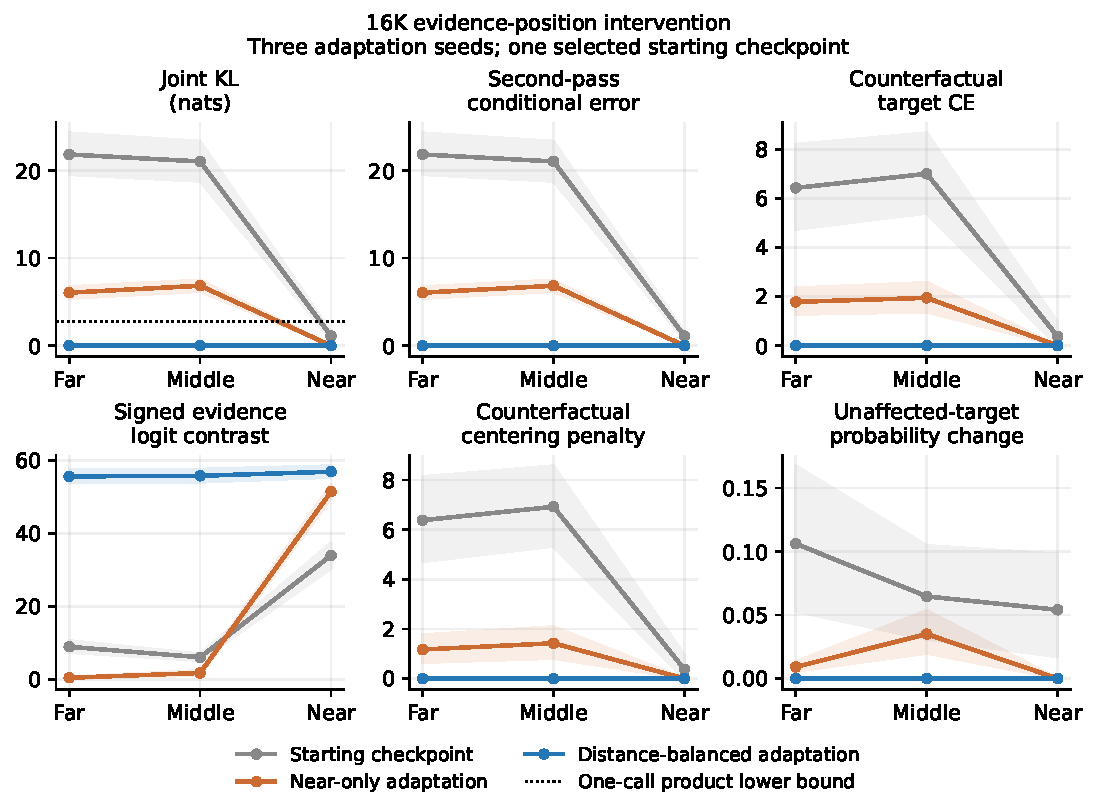
\includegraphics[width=\linewidth]{results/distance_intervention/mechanism_distance_paper.pdf}
\caption{Matched 16K distance intervention. Curves average the three adaptation
seeds within each of 32 paired problems; shading gives pointwise 95\%
problem-bootstrap intervals, conditional on the selected lineage and these
seeds. The starting checkpoint is descriptive. The top-left dotted line is
the one-call product lower bound. Endpoint error integrates all target
histories; counterfactual panels use the declared fixed visible history.
Numerically small balanced errors are shown explicitly in the tables.}
\label{fig:distance}
\end{figure}

\paragraph{The advantage survives nearby instructions and distant task information.}
A frozen follow-up separates the generic instruction header from the task block
on 32 fresh prompts, testing four fixed-slot layouts and two legacy controls
(Appendix~\ref{app:header-distance}). With the header nearby and the task block
far away, balanced training reduces conditional error by 7.6266 nats
$[6.9081,8.3015]$, positive in every seed. Every balanced model's mean error
is below $0.000153$ nats in that cell. Both arms remain accurate with nearby
task information even when the header is distant. However, regrouping
irrelevant records changes one near-trained model's mean far error by 4.09
nats. The result supports the advantage under these declared layouts, not
layout invariance. The task block includes names and output-order metadata;
this inference intervention does not separate the components of the training
treatment, and intervals still condition on the same selected lineage.

\paragraph{The learned equal-call contrast matches the dependence prediction.}
Across the three 16K positions, balanced information-set KL is 0.000199,
0.000009, and 0.000257 nats for the three seeds. The intact-pair minus
information-set contrast is 2.772465, 2.772605, and 2.772696 nats. Its difference
from the predicted $4\log2$ is at most $1.24\times10^{-4}$ nats in absolute
value. Thus the observed mean contrast is dominated by the prescribed
dependence reduction once both conditional policies are competent.
This conclusion requires the measured $E$ values: near-only models have
estimation-error differences from $-4.804$ to $-1.848$ nats, so their equal-call
contrasts cannot be attributed to $D$ alone (Table~\ref{tab:distance-cost}).

\paragraph{The matched budget certificate holds for all balanced selectors.}
On the separate eight-problem quality--cost panel, recurrent two-call times
are 1.301--1.307 seconds across all six models. Attention costs 1.003 seconds
for one call, 2.002 for information-set two-call execution, and 2.003 for
intact-pair two-call execution. The predeclared 1.5-second mean budget therefore
permits recurrent two-call and attention one-call execution while excluding
both other declared attention policies. All balanced models have matched KL
below $4\log2$, so all three meet the empirical sufficient certificate.
Two near-only models fail its quality condition. The third passes the
aggregate certificate because accurate nearby queries offset near-chance
far and middle predictions; it still has far KL 2.7725. This distinction is why
the primary mechanism test specifies the distant position instead of relying
only on an aggregate score.

\begin{table}[t]
\centering\small
\caption{All fixed adaptations. The 16K KL and equal-call gain average 32
problems and three positions. Equal-call gain is intact-pair minus
information-set KL; its dependence-only prediction is $4\log2$.
Matched KL, latency, and certificate use the separate eight-problem,
three-position panel and the 1.5-second mean budget. All KL values are nats.}
\resizebox{\linewidth}{!}{\begin{tabular}{llrrrrl}
\toprule
Arm & Seed & 16K KL & Equal-call gain & Matched KL & Two-call (s) & Certificate \\
\midrule
Near-only & 20271011 & 6.1875 & -1.6543 & 5.2300 & 1.301 & Fail \\
Balanced & 20271011 & $1.99\times10^{-4}$ & 2.7725 & $6.31\times10^{-4}$ & 1.302 & Pass \\
Near-only & 20271012 & 4.8595 & -2.0313 & 4.5207 & 1.307 & Fail \\
Balanced & 20271012 & $9.07\times10^{-6}$ & 2.7726 & $4.33\times10^{-6}$ & 1.306 & Pass \\
Near-only & 20271013 & 1.8482 & 0.9244 & 1.8483 & 1.301 & Pass \\
Balanced & 20271013 & $2.57\times10^{-4}$ & 2.7727 & $9.29\times10^{-5}$ & 1.302 & Pass \\
\bottomrule
\end{tabular}
}
\label{tab:distance-cost}
\end{table}

The certificate uses the analytic product-predictor lower bound, not measured
attention answer quality. It supplies no per-request deadline guarantee and
does not exclude optimized alternatives or cached causal decoding.
Peak allocated inference memory is 4.125 GiB for RWKV and 2.234 GiB for attention;
this implementation demonstrates no memory advantage.
The exploratory eight-problem 32K far panel has balanced KL below 0.00041
in all three seeds, but it does not establish general extrapolation beyond
the tested lengths. All secondary cells are retained in
Appendix~\ref{app:distance-supplement}.
